% Signal comparison (audit F-1 corrected): DIRECT AUROCs with 95% bootstrap CIs.
% The convergence residual is kappa = v1/vS (first/last). The original vS/v1 is inverted on our data.
\documentclass[border=6pt]{standalone}
\usepackage[T1]{fontenc}
\usepackage{helvet}
\renewcommand{\familydefault}{\sfdefault}
\usepackage{tikz}
\usepackage{pgfplots}
\pgfplotsset{compat=1.18}
\usepackage{xcolor}
\definecolor{t4c}{HTML}{1668D6}
\definecolor{a100c}{HTML}{B26A00}
\definecolor{mut}{HTML}{5A6B80}

\begin{document}
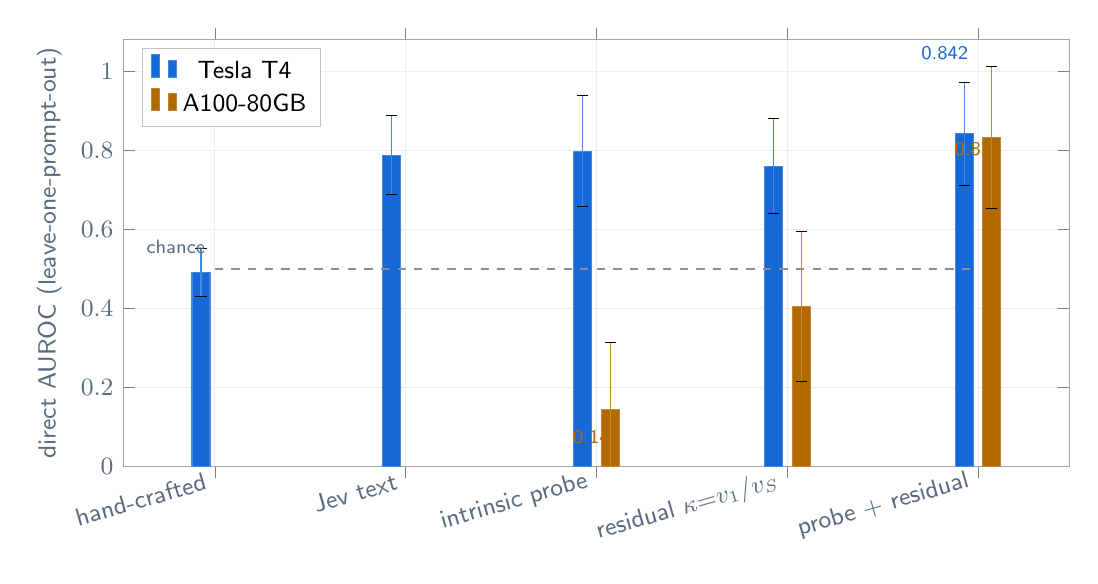
\begin{tikzpicture}
\begin{axis}[
  width=13.6cm, height=7.0cm,
  ybar, bar width=6.5pt, bar shift=0pt,
  ylabel={direct AUROC (leave-one-prompt-out)},
  symbolic x coords={hand-crafted, Jev text, intrinsic probe, residual $\kappa{=}v_1/v_S$, probe + residual},
  xtick=data, x tick label style={font=\small,rotate=16,anchor=east,color=mut},
  ymin=0.0, ymax=1.08, ytick={0,0.2,0.4,0.6,0.8,1.0},
  tick label style={font=\small,color=mut},
  label style={font=\small,color=mut},
  axis line style={draw=mut!60},
  legend style={font=\small,at={(0.02,0.98)},anchor=north west,draw=mut!40,fill=white},
  grid=major, grid style={draw=mut!12},
  enlarge x limits=0.12,
  error bars/y dir=both, error bars/y explicit,
]

% Tesla T4  (bar shift -5pt)
\addplot[fill=t4c,draw=t4c!80,bar shift=-5pt,
  error bars/.cd, y dir=both, y explicit]
  coordinates {
  (hand-crafted,0.491) +- (0,0.06)
  (Jev text,0.788) +- (0,0.10)
  (intrinsic probe,0.798) +- (0,0.14)
  (residual $\kappa{=}v_1/v_S$,0.760) +- (0,0.12)
  (probe + residual,0.842) +- (0,0.13)};

% A100-80GB  (bar shift +5pt)
\addplot[fill=a100c,draw=a100c!80,bar shift=+5pt,
  error bars/.cd, y dir=both, y explicit]
  coordinates {
  (intrinsic probe,0.143) +- (0,0.17)
  (residual $\kappa{=}v_1/v_S$,0.404) +- (0,0.19)
  (probe + residual,0.833) +- (0,0.18)};

\draw[mut!75,dashed,line width=0.5pt] (axis cs:hand-crafted,0.5) -- (axis cs:probe + residual,0.5);
\node[font=\scriptsize,color=mut,anchor=south east] at (axis cs:hand-crafted,0.515) {chance};

\node[font=\scriptsize,color=t4c,anchor=east]   at (axis cs:probe + residual,1.045) {0.842};
\node[font=\scriptsize,color=a100c,anchor=north] at (axis cs:probe + residual,0.845) {0.833};
\node[font=\scriptsize,color=a100c,anchor=north] at (axis cs:intrinsic probe,0.115) {0.143};

\legend{Tesla T4, A100-80GB}
\end{axis}
\end{tikzpicture}
\end{document}
